\chapter{Task, Motion and Manipulation Planning}
\label{chapter: task_and_motion_planning}
\textit{
This chapter will provide an overview of different \textbf{\ac{TAMP}} methods. In the previous chapter, \cref{chapter: interaction_with_env_and_model_identification} the nonlinear nature of single-body, but especially multi-body systems was shown. The constraints due to the nonholonomic nature of the robot is captured in system models, system models will assist as local planners during motion and manipulation planning. Motion planning discussed in \cref{section: toward_target_pose} is conveniently split in a part for single bodies in \cref{subsection: motion_planning} and a part for multi-bodies in \cref{subsection: manipulation_planning}. Decidability of motion and manipulation planners is analysed in \cref{subsection: path_existence}. Solutions to a given task seldom exist of a single motion. For multiple motions, the effects of a motion executed propagates further to future task planning. Such arisen problems related to \ac{TAMP} and possible solutions are discussed in \cref{section: toward_sequence_target_poses}. Performance and limitations are discussed in \cref{section: tamp_discussion}.
}\\

\section{Toward a Target Pose}
\label{section: toward_target_pose}
Decades of research yield a numerous amount of path-finding algorithms for many different applications \cite{lavalle_planning_2006,karaman_sampling-based_2011}. Such a broad field of research is lessened down to methods applicable to robotic applications. Before moving further, let's first clarify the configuration space and motion planning. The  \textit{configuration space} is a set of possible transformations that could be applied to the robot \cite{lavalle_planning_2006}. A robot can be described as a point in configuration space, which is a robot's \textit{configuration}. From the robot's dimensions and it's configuration all points of the robot can fully be described. The configuration space consists of the non-overlapping obstacle space and free space. The robot can encounter obstacles which should be avoided, obstacles are represented in the \textit{obstacle space}. The robot is allowed in \textit{free space}, represented as a set of configurations in configuration space, and not in the obstacle space. Finally, motion planning is, given 2 robot configurations in free space, finding a feasible path between such 2 robot configurations. Two examples clarifying motion planning are presented in \cref{figure: single_body_motion_task,figure: multi_body_motion_task}. Motion planning is split into 2 categories, motion planning for single-bodies and motion planning for multi-bodies also called \textit{manipulation planning}. \\

 
\subsection{Motion Planning}
\label{subsection: motion_planning}
\Cref{figure: single_body_motion_task} displays a 2D representation of a motion planning task. In this example, the configuration space is 3-dimensional containing position and orientation (x, y and $\theta$). In configuration space, a path between the starting and target configuration should be found while avoiding obstacles and respecting constraints. While learning object dynamics, motion planning should be performed while having access to partly known or unknown robot dynamics, translating into partly known or unknown knowledge of constraints. With limited knowledge of constraints, motion planners might tend to find paths infeasible for the robot to track. For example, a feasible path found without full knowledge of the constraints could actually be unfeasible. Model mismatch might also yield unfeasible paths, and might prevent finding feasible paths. Again stressing the importance of system models. As a rule of thumb, respect known constraints, expect unknown constraints. Recent literature on the topic of motion planning with constraints is a subject which has had a considerable amount of research \cite{kingston_sampling-based_2018,lavalle_planning_2006}. The most prominent are sampling-based methods and graph-based methods which will now be discussed. 

\paragraph{Sample-Based Planners}

\begin{figure}[h!]
    \centering
    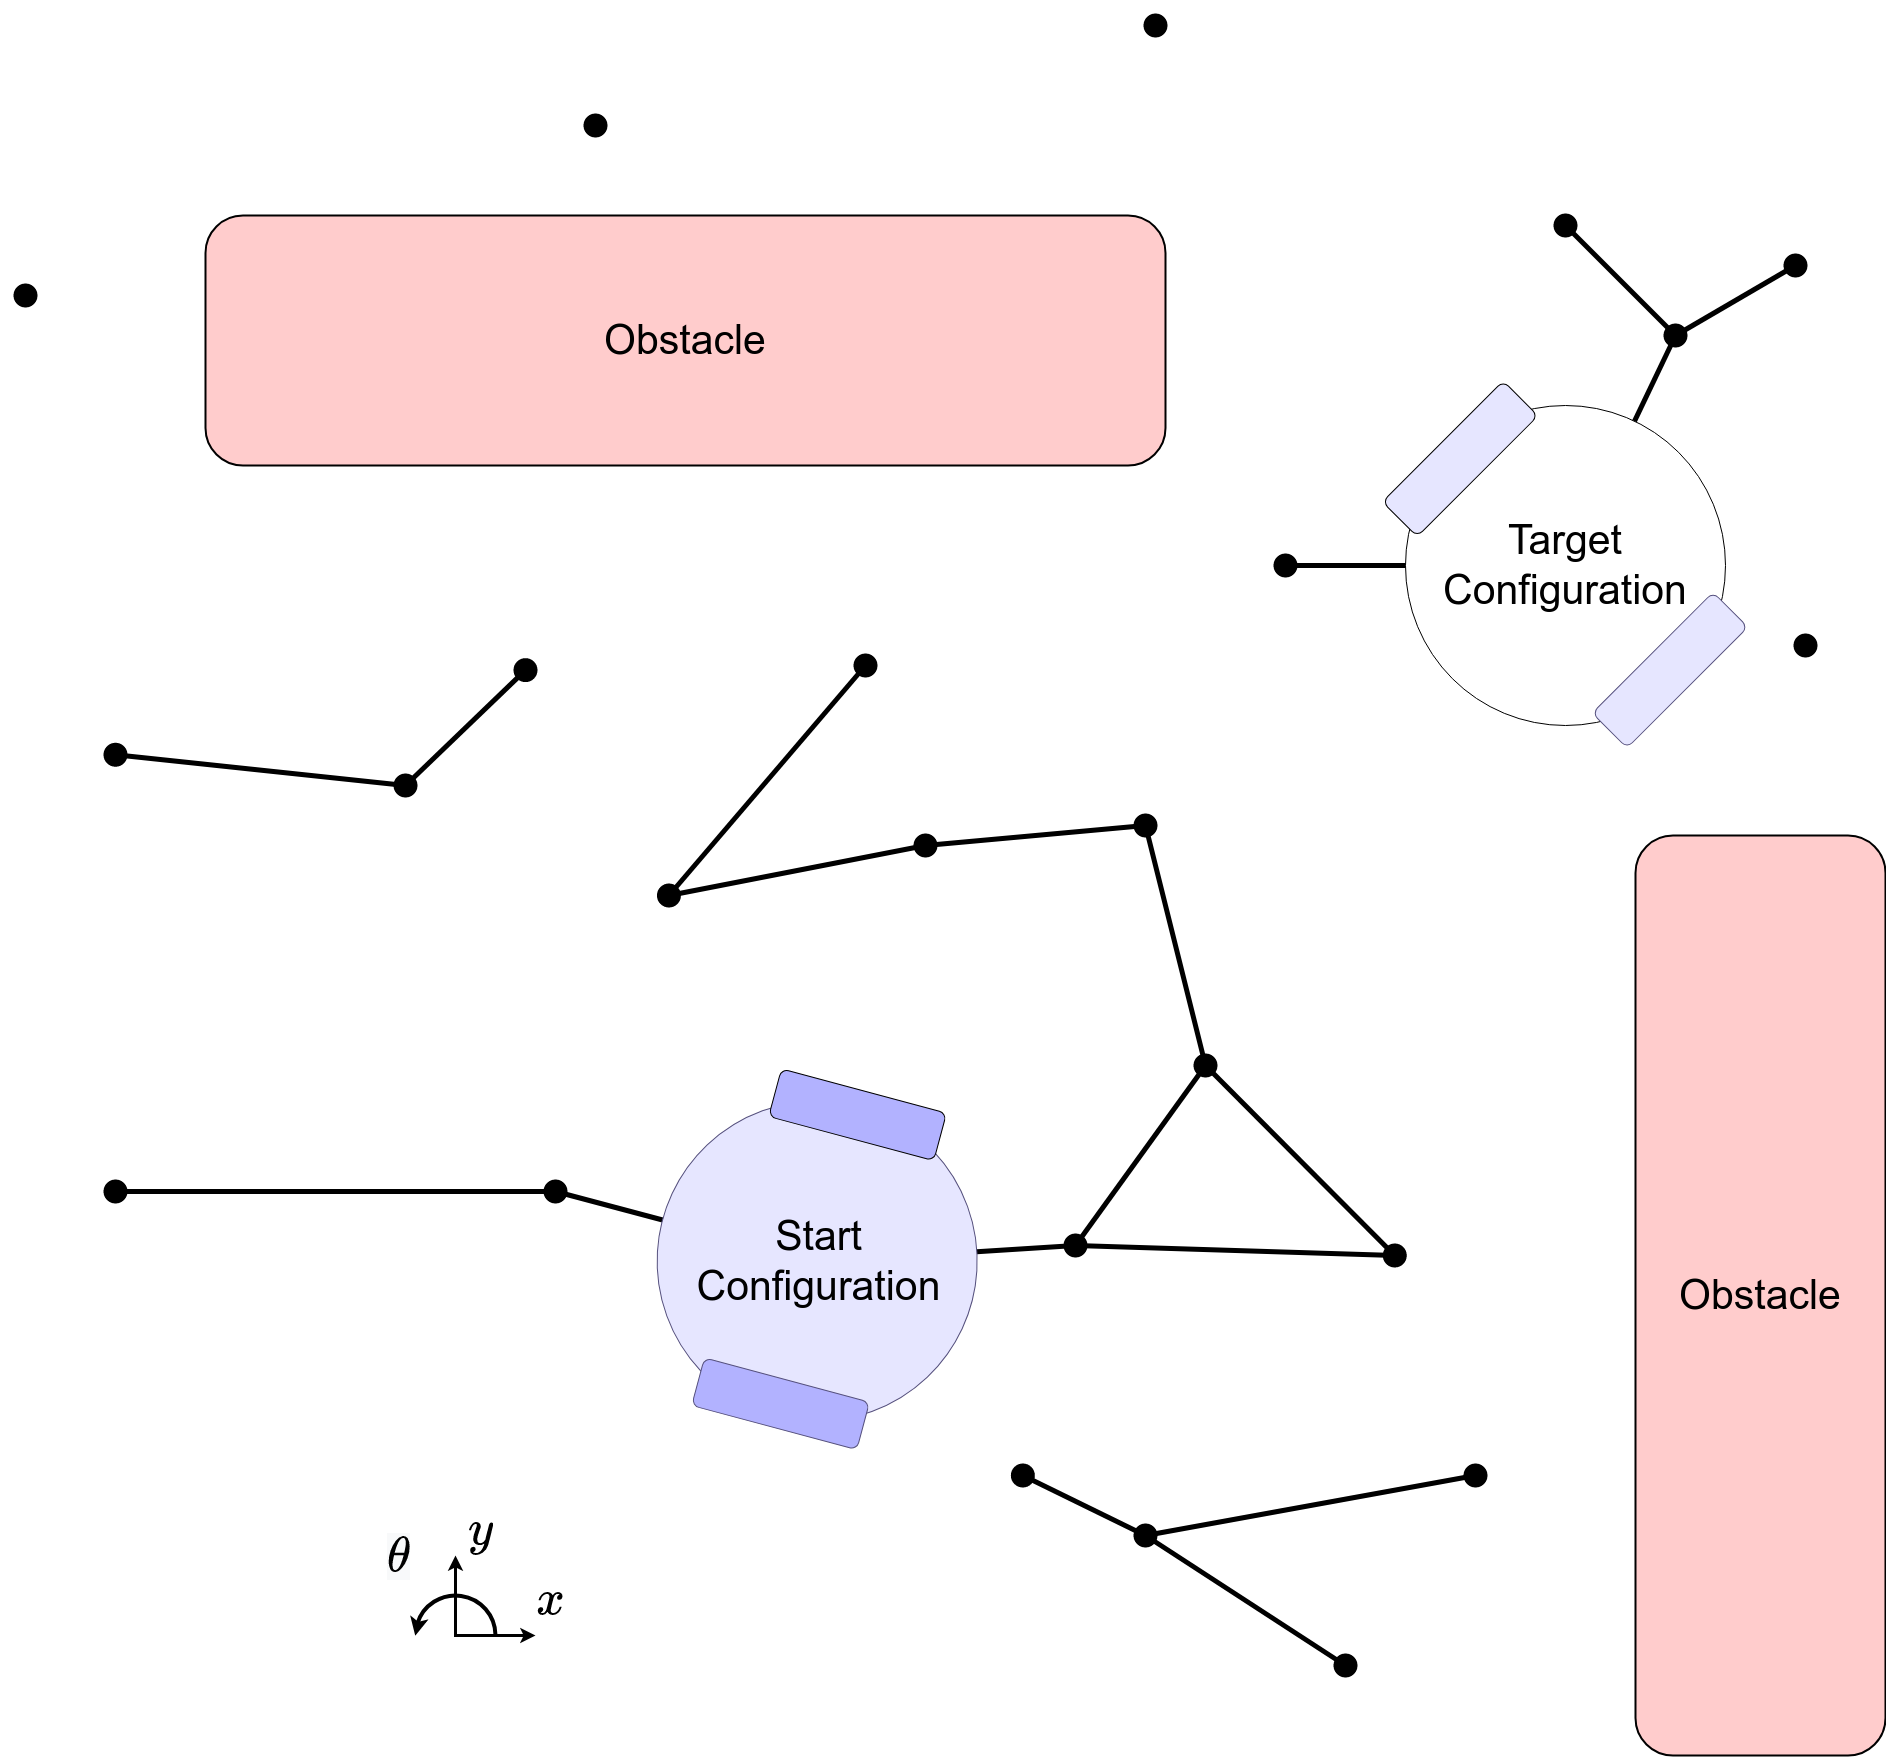
\includegraphics[width=0.7\textwidth]{figures/motion_planning_robot.png}
    \caption{Sample-based motion planning task including 2 obstacles, a start and target configuration and a visual representation of sampled configurations with the connectivity graph}
    \label{figure: single_body_motion_task}
\end{figure}

The general idea behind sampling-based planning is to avoid computing the free space exactly and instead sample configurations in free space and connect them to construct a tree or graph that approximates the connectivity of the underlying free space \cite{kingston_sampling-based_2018}. To connect 2 sampled points, a one- or multi-step-ahead predictor must be able to connect both, such a predictor is also commonly called a local planner in vast literature, a \textit{connectivity graph} indicates sampled configurations which are verified by a local planner, an visual example for manipulation planning can be seen in \cref{figure: local_planner_manipulation}. Using learned single-body models and one-step-ahead predictors discussed in \cref{chapter: interaction_with_env_and_model_identification} sampled points in configuration space can be connected. For a sampling-based planner to plan with constraints, sampling and local planning must be augmented to satisfy constraints, as both of these elements directly affect whether the planning generates a valid path; as such, most methods focus on these two elements \cite{kingston_sampling-based_2018}. \\

Even with infinite sampling, the optimal path could be withheld because model mismatch does not allow the optimal path to be found. Logically a motion planner validating constraints using a nonsense local planner, will (most probably) not find the optimal path or will find a path which in reality is unfeasible. The overwhelming majority of solution techniques are sampling-based. This is motivated primarily by the extreme difficulty of planning under differential
constraints \cite{lavalle_planning_2006}, such as constraints due to nonholonomic nature of the robot. Chapter 14 from LaValle \cite{lavalle_planning_2006} is a interesting read on sampling-based planner under differential constraints. Contains a classification of planning problems, reachability guarantees, and various metrics to sample into a direction toward the target configuration.\\

Notably, most techniques for constrained sampling-based motion planning do not alter the core mechanics used by sampling-based planners. Generally, constrained sampling-based algorithms are adaptations of existing algorithms that incorporate a methodology for constraint satisfaction \cite{kingston_sampling-based_2018}. Local planners provided by system models provide a validator for constraint satisfaction, it is thus now sufficient to look at motion planners without constraints and complement them with local planners. A summary of sampling-based is displayed in \cref{fig: summary_sampling_based_methods}, where a formal analysis is done of most prominent sampling-based methods, such as \ac{PRM} and \ac{RRT} and \ac{RRT}\textsuperscript{*}.

%% TABLE %%%
\begin{table}[H]
\centering
\ra{1.3}
\begin{tabular}{@{}c|cccccc@{}}
\shortstack[]{\textbf{Algorithm}} & \multicolumn{1}{c|}{\shortstack[]{Probabilistic\\Completeness}} &
\multicolumn{1}{c|}{\shortstack[]{Asymptotic\\Optimality}}&
\shortstack[]{Monotone\\Convergence} &
\multicolumn{2}{|c|}{\shortstack[]{Time Complexity\\Processing \hspace{0.4cm}|\hspace{0.5cm} Query}} & \shortstack[]{Space\\Complexity}\\
\midrule
PRM & \cmark & \xmark & \cmark & $\mathcal{O}(n\log{}n)$ & $\mathcal{O}(n\log{}n)$ & $\mathcal{O}(n)$\\
\ac{RRT} & \cmark & \cmark & \cmark & $\mathcal{O}(n^2)$ & $\mathcal{O}(n)$ & $\mathcal{O}(n^2)$\\
\ac{RRT}\textsuperscript{*} & \cmark & \cmark & \cmark & $\mathcal{O}(n \log(n))$ & $\mathcal{O}(n)$ & $\mathcal{O}(n^2)$\\
\bottomrule
\end{tabular}
\caption{Summary on sampling based methods with space and time complexity as function of the number of samples $n$ in a fixed environment,  from \cite{karaman_sampling-based_2011}}
\label{fig: summary_sampling_based_methods}
\end{table}

A challenge in robotics is the convergence speed at which a path is found. Ideally, path finding is fast enough, such that the robot can continuously operate. Increasing convergence speed can be attained by implementing a faster algorithm or by applying techniques to improve the local planner. \\

One method to speed up convergence is to add sampled configurations to the connectivity graph starting from both the starting and target configuration, applied by \cite{chen_fast_2018} who showed that \ac{RRT}\textsuperscript{*} with double-tree it outperformed existing \ac{RRT}\textsuperscript{*}. Techniques to speed up local motion planners are beautifully categorised in \cite{kingston_sampling-based_2018} two major techniques are \textit{relaxation} where constraints are allowed to be broken for a small threshold to find feasible paths faster. The other major technique is \textit{projection} where an infeasible sampled configuration is projected onto the feasible region. \cite{kingston_sampling-based_2018} explains these concepts in more elaborate and lists techniques such as tangent space, atlas or reparameterisation which all help to increase convergence. \\

\paragraph{Graph-Based Planners}

\begin{figure}[H]
    \centering
    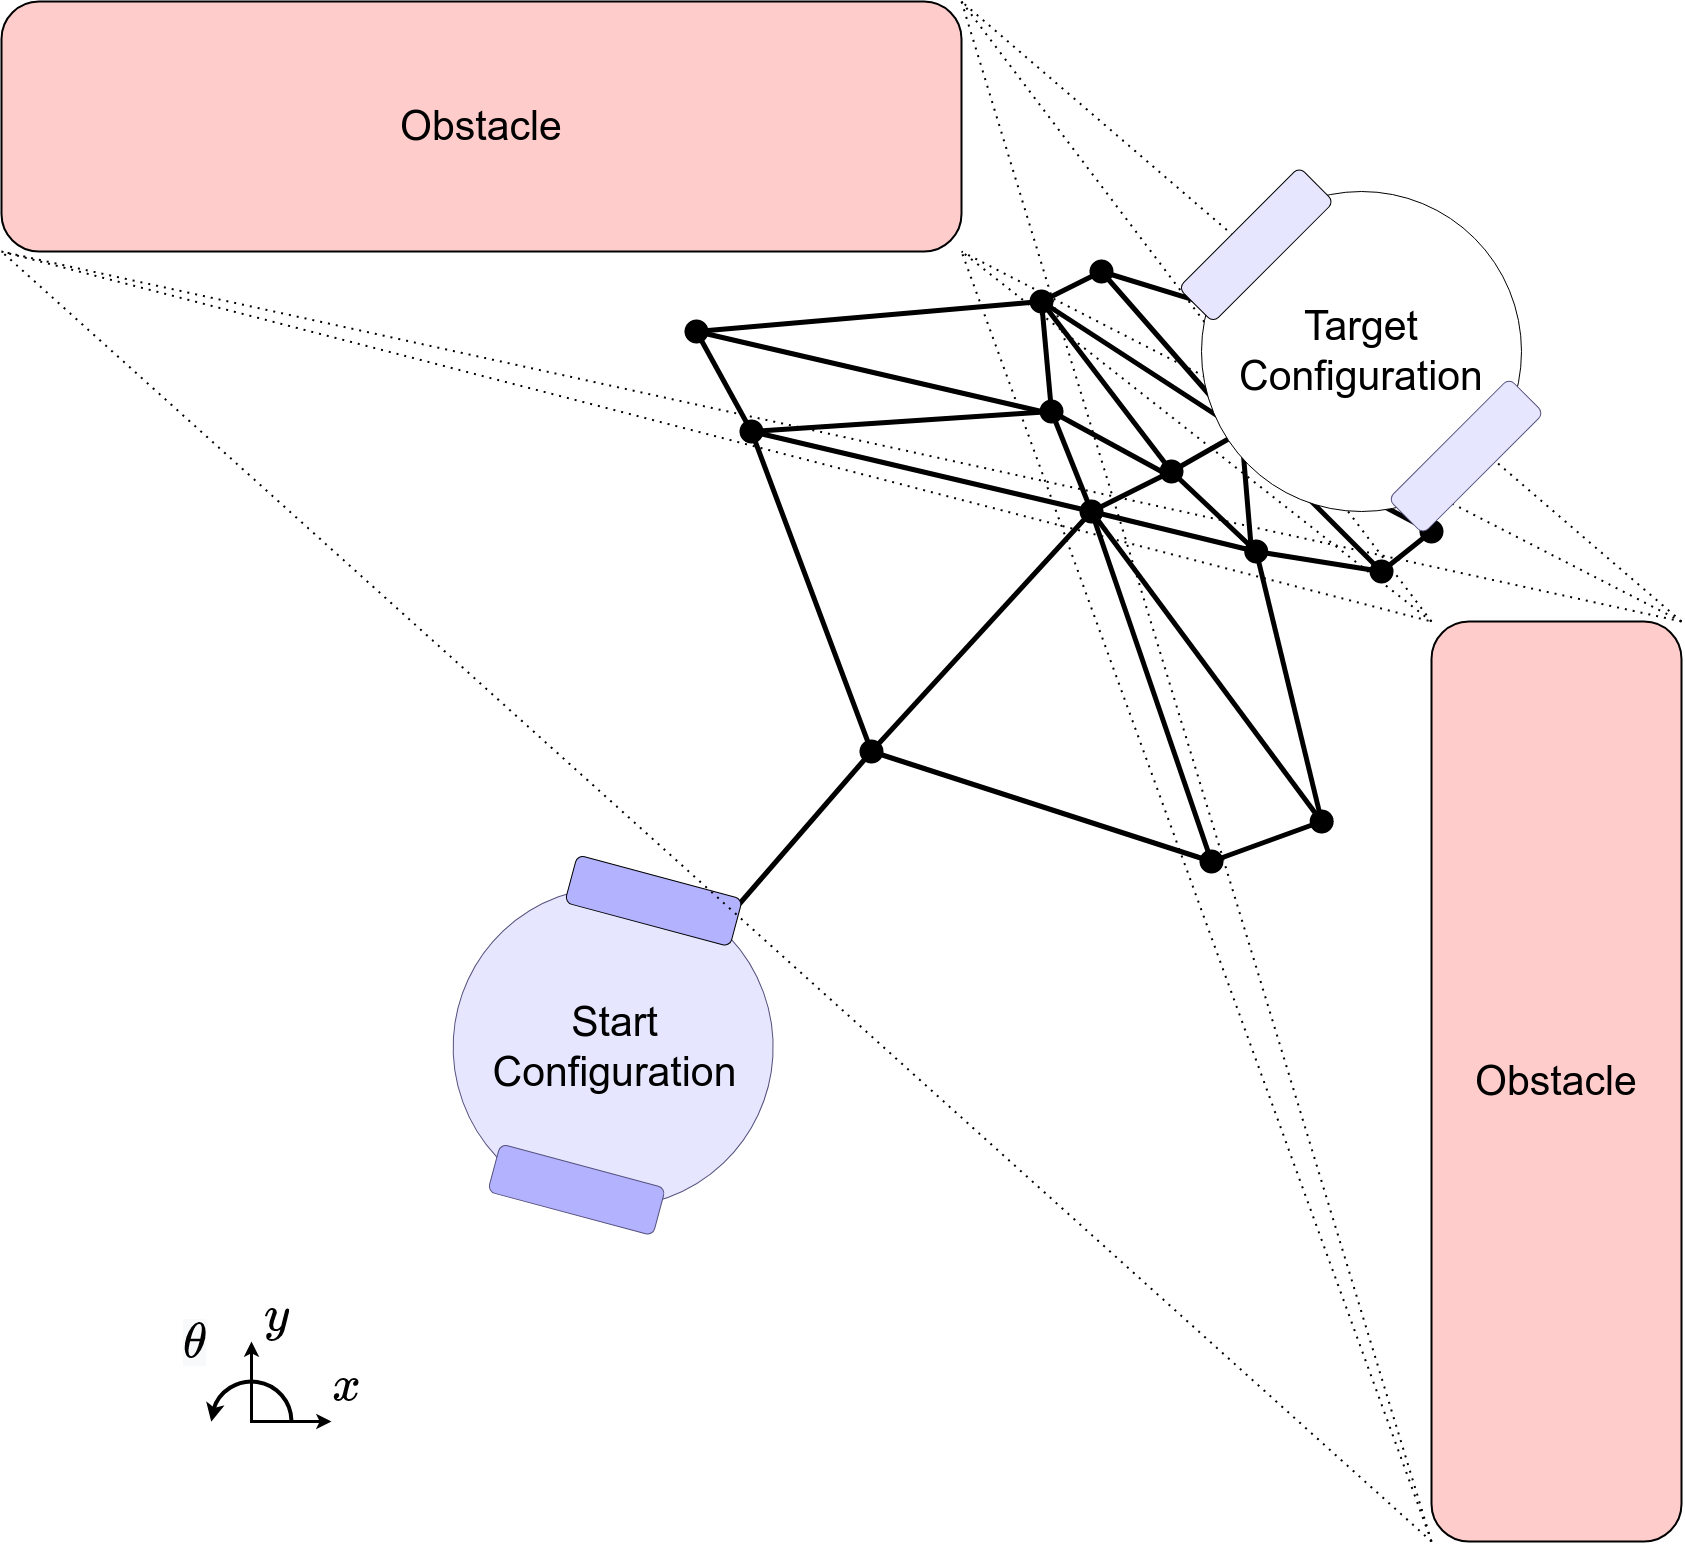
\includegraphics[width=0.7\textwidth]{figures/robot_motion_planning_graph.png}
    \caption{Graph-based motion planning task including 2 obstacles, a start and target configuration and a visual representation of graph-based configurations with the connectivity graph}
    \label{figure: single_body_motion_task_graph}
\end{figure}

An alternative to sampling-based methods is a finite discretization (with for example a grid, or a cell decomposition) of the configuration space.  Which gives rise to \textit{graph-based} search algorithms such as: $\text{A}^*$ and Dijkstra \cite{karaman_sampling-based_2011}. However because the number of grid points grows exponentially with the dimensionality of the configuration space, so does the worst-case running time. Which is the reason that randomisation is so powerful when exploring high-dimensional search spaces. \\ 

When the dimensionality of the configurations spaces increases, the time it takes to fully discretize grows exponentially. Only after a full discretezation, a graph-based search can start. Where as sample-based planners which can immediately start sampling configurations. In high-dimensional configuration spaces a graph-based methods take a comparatively longer time then sample based methods because of the required discretezation period, thus sample-based methods are the better choice for motion planning. When the system model converges toward the true dynamics, the local planner improves as a result, and the motion planner will yield more feasible paths. Graph-based planners will not play a role during planning but can provide a solution to another problem discussed in \cref{subsection: path_existence}.

\subsection{Manipulation Planning}
\label{subsection: manipulation_planning}
Manipulation planning differs from motion planning in a few aspects. Recall that manipulation planning is motion planning for multi-body systems, whereas motion planning refers to planning for a single-body system. With multi-body systems, one body (the robot) is controlled which indirectly controls the object when the robot pushes, pulls or picks the object, the robot is manipulating the object. Generally, with motion planning there is prior knowledge about the robots dynamics and constraints available, with manipulation planning there exist more constraints, which are lesser known, depending on the amount of system identification performed on the specific robot-object combination. \\

Let's consider the example manipulation planning task in \cref{figure: multi_body_motion_task}, here both the robot and the cube object are in the starting configuration represented in configuration space again consisting of $X$, $Y$ coordinate and orientation $\theta$. Manipulation tasks are completed as the object is in the desired position, the robots target configuration is irrelevant. Constraints which must be respected are the single-body constraints from the robot and the object, the multi-body constraints and that all configurations must be in free space. \\

For a configuration the object is in, infinite possibilities exist for the robot to be in, resulting in a exponential explosion of the number of possible configurations. Such a configuration space of the robot and objects is referred to a joint configuration space. Directly searching the joint configuration space is unwise because the number dimension is to high to find a path in reasonable time (far from real-time motion planning). Even so planning in a joint configuration space is shown to be successful, by implementing enormous simplification, \cref{subsection: planning_in_joint_config} discusses the joint configuration space more extensive.\\

In recent literature many push manipulations simplify pushing by using an holonomic pusher (e.g. a controlled stick) instead of an nonholonomic robot \cite{bauza_data-efficient_2018,kopicki_learning_2017,cong_self-adapting_2020,arruda_uncertainty_2017}. If manipulation planning is performed with the use of a nonholonomic robot, other measured must be taken to counter the computational expensive search. \\

\begin{figure}[H]
    \centering
    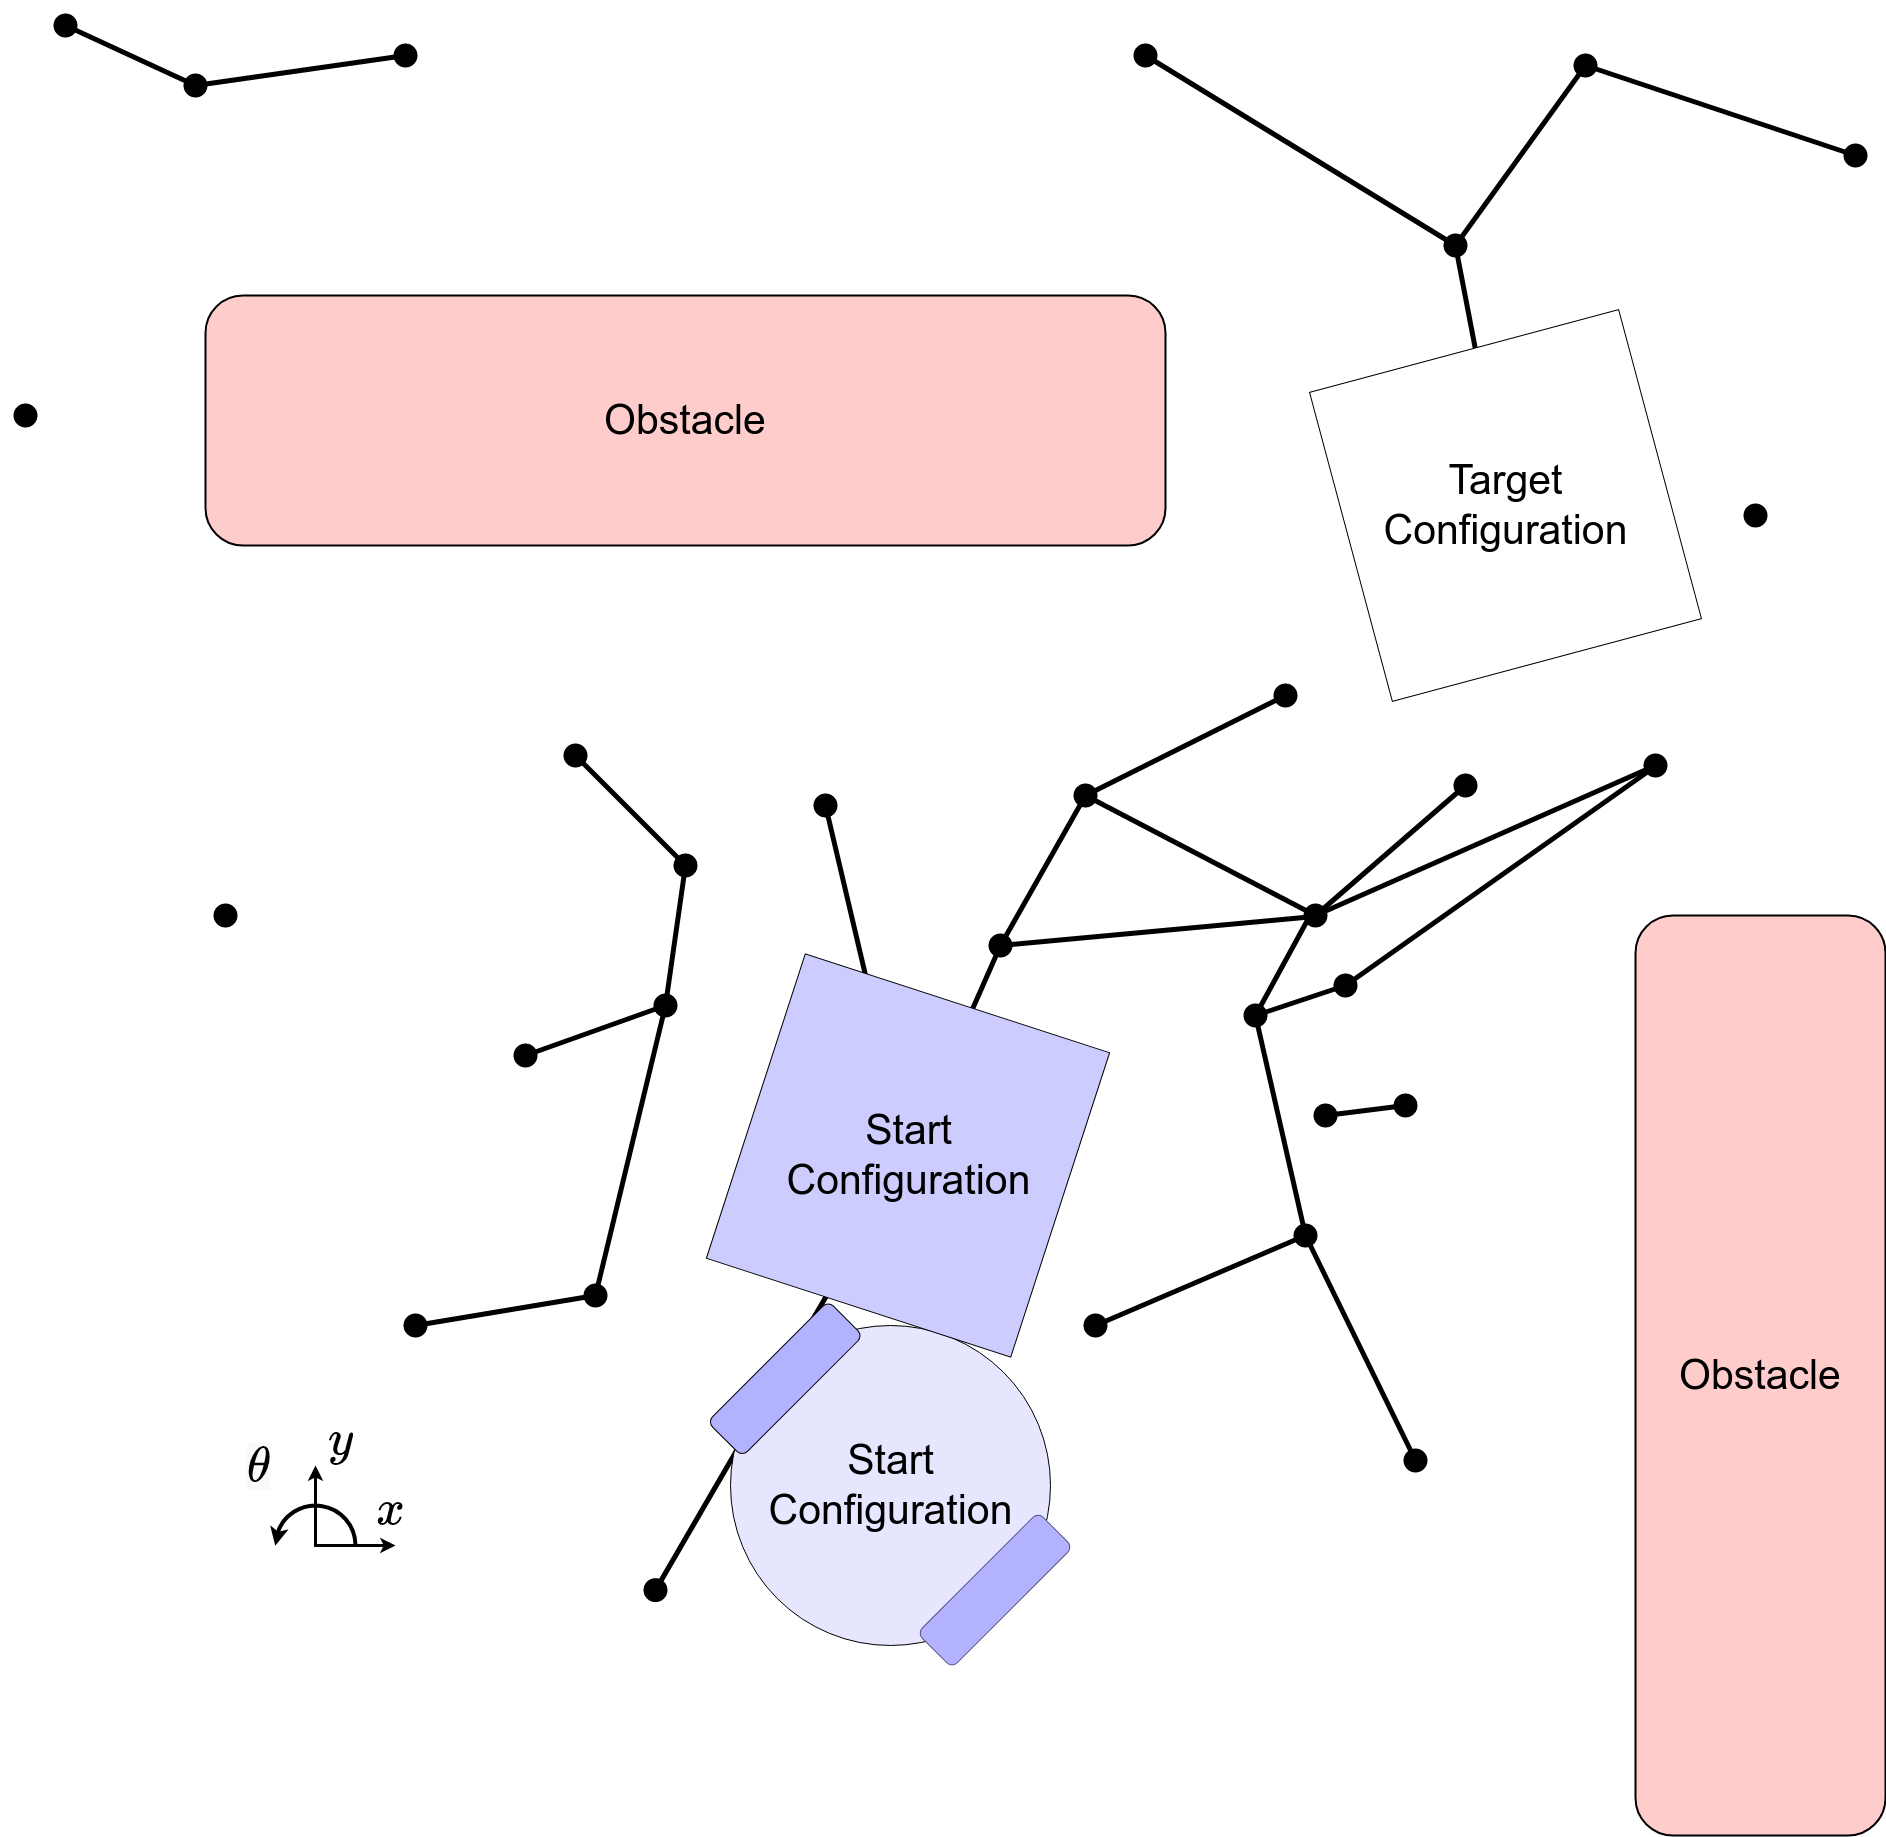
\includegraphics[width=0.7\textwidth]{figures/motion_planning_robot_and_square_object.png}
    \caption{Manipulation planning task, to push the box toward the target configuration, including 2 obstacles, sampled configurations and the connectivity graph}
    \label{figure: multi_body_motion_task}
\end{figure}

The paper \cite{mericli_push-manipulation_2015}, already discussed in \cref{subsection: predictive_methods,subsection: data_driven_models} for it's data-driven model and model identifying method, provides a \ac{RRT} algorithm which uses the experimentally acquired model. An example simplification of the search space would be to only use large test pushes during data collection. Large test pushes only results in a local planner connecting 2 configuration with large pushes only. The planner then finds a path consisting of multiple large pushes and not a continuous push, as a result a path will be tracked by multiple pushes where the object comes at a complete stop after every push, which is far for optimal. While \cite{mericli_push-manipulation_2015} managed to create a stable planner for a data-driven model identifying method, the push manipulation is far from optimal because the local planner is unable to produce a continuous push. \\

A simplification can be made forcing a multi-body into a single body, achieved by gripping an object with 2 grippers and then planning for a single-body model \cite{scholz_navigation_2016}. During execution \cite{scholz_navigation_2016} learns the multi-body model consisting of the robot and a gripped object. \cite{scholz_navigation_2016} detects an immovable object or an object that is immovable in an subspace of its configuration space by comparing predicted with measured outcome. Detection can differ between an completely immovable object, or an partly immovable object (e.g. it can only rotate but not translate), which is made possible by checking prediction errors per subspace dimension.\\

Converting manipulation planning completely to motion planning simplifies the problem considerably. \cite{arruda_uncertainty_2017} neglects the pusher, plans only for motion of the object, the robot pusher is then tasked with manipulating the object such that it tracks the found path with an \ac{MPPI} controller. Such a strategy requires additional measures to counter the neglected constraints imposed by the multi-body model and the starting configuration of the pusher. In \cite{arruda_uncertainty_2017} case this is done by planning a push in the direction with high model certainty, but most hard constraints can be neglected because the robot is an holonomic push arm and not an nonholonomic robot. \\

Using multiple methods to speed up computation, R. Sabbaragh Novim e. al. developed an dedicated search algorithm for path finding of single- and multi-body model \cite{sabbagh_novin_optimal_2016}.  Methods used are discretisation of the configuration space, a receding planning horizon which allows planning toward the target, but prevent planning all the way up until the target. Sabbaragh proceeds to use his algorithm in an hospital setting, in which a robot with gripper is tasked to bring walking aid to patients who request it \cite{novin_dynamic_2018}. Improving upon his own work 2 years later, adding improved model identification methods allowing a larger variety of object to manipulate \cite{sabbagh_novin_model_2021}.\\

For manipulation planning recent literature has made one thing very clear, direct planning in a multi-body configuration space is computationally infeasible. Sample-based planners are a valid manipulation planning strategy as long as the multi-body configuration space is avoided. Thus a simplification of the joint configuration space is required. A few recently used simplifications are discretising by allowing only a small selection of pushes, gripping an object creating a single body, considering only the object to push during planning or planning toward the target without planning the path entirely. The bulk of manipulation planners are sample based. The $\text{RRT}^*$ algorithm is preferred because it is a sample-based planner, probabilistic complete and has a favourable time complexity. 

\subsection{Path Existence}
\label{subsection: path_existence}
The standard Piano Mover’s Problem is PSPACE-hard \cite{reif_complexity_1979}, motion planning is PSPACE-hard \cite{canny_complexity_1988}, optimal planning is NP-hard  \cite{canny_new_1987}, the only known methods for exact planning under differential constraints in the presence of obstacles is for a double integrator system $\ddot{x} = u$, with $x$ the state and $u$ the input \cite{lavalle_planning_2006}.  Aiming for an optimal solution in motion or manipulation planning with differential constraints is clearly out of the question, the point is that path planning is practically undecidable. With exeptions for linear systems and a dublin's car where motion planning is found to be decidable\cite{cheng_decidability_2007}, unfortunately such systems are not the scope of this literature. For any motion planning task any of the two outcomes is true, there exist a path from start to target and searching for it makes sense, or there does not exist a path from start to target and searching for it is meaningless. Especially for sampling-based methods, where without a stopping criteria, the sampling algorithm keeps on sampling. Of course a certain threshold can be set, but then the next difficult question arises, what threshold to set? It is thus worth searching for existence or non-existence of a path, proving path existence requires searching for a path with infinite sampling, which is impossible. But path non-existence can in some cases be detected, for example if a piano physically does not fit through a door (assuming the door is the only path and no other exists). Knowledge of non-existence of a path reduces the search space. One such example is caging, where a robot is trapped, which is proven to be detectable \cite{amato_caging_2020}.\\

For \textit{holonomic} robots, checking for path path-existence can be estimated by discretizing the configuration space with the obstacles while accounting for the robot's dimensions \cite{akella_simple_2008}. The estimation becomes more reliable if the grid size at discretization decreases. Graph-based algorithms such as $\text{A}^*$ can find a path from start to target cell, or halt when no path exists for a finite graph. If no path exist for a holonomic version of the robot, then there does also not exist a path for the nonholonomic robot. If there exist a path for the holonomic robot, it might not exist for the nonholonomic version of the robot. The configuration samples from the grid cell can be used as a "warm start" during motion or manipulation planning. In the case a path exists for the holonomic version of a nonholonomic robot, a path will be most likely found during a check for path non-existence, but will not be found during motion or manipulation planning, even if the same samples from the path existence algorithm are used as a warm start. \\

The importance of estimating path existence has been pointed out. Non-existence of a path can be proven, and path-existence can be estimated. Simple checks such as suggested by \cite{akella_simple_2008} can prevent unnecessary calculations. 

